\documentclass[12pt]{article}
\usepackage{algorithmicx}
\usepackage[ruled]{algorithm}
\usepackage{algpseudocode}
\usepackage{algpascal}
\usepackage{algc}
\usepackage{url,enumerate, amssymb, anysize, booktabs, amsfonts}
\usepackage[colorlinks = true,
linkcolor = blue,
urlcolor  = blue,
citecolor = green,
anchorcolor = blue]{hyperref}
\usepackage{setspace,listings}
\usepackage[dvipdfmx]{graphicx}
\usepackage{amsmath}
\usepackage{psfrag}
\usepackage[font=small,labelfont=bf]{caption}
\usepackage{enumerate}
\usepackage{natbib}
\usepackage{url} % not crucial - just used below for the URL 


\begin{document}
	
	\title{Outline of \\``Testing independence between networks and nodal attributes via multiscale metrics''}
	
	\author{Youjin Lee}
	
	\maketitle
		
%%%%%%%%%%%%%%%%%%%%%%%%%%%%%%%%%	
\subsection*{1. Introducing network topology}

\begin{figure}[H]
	\centering
	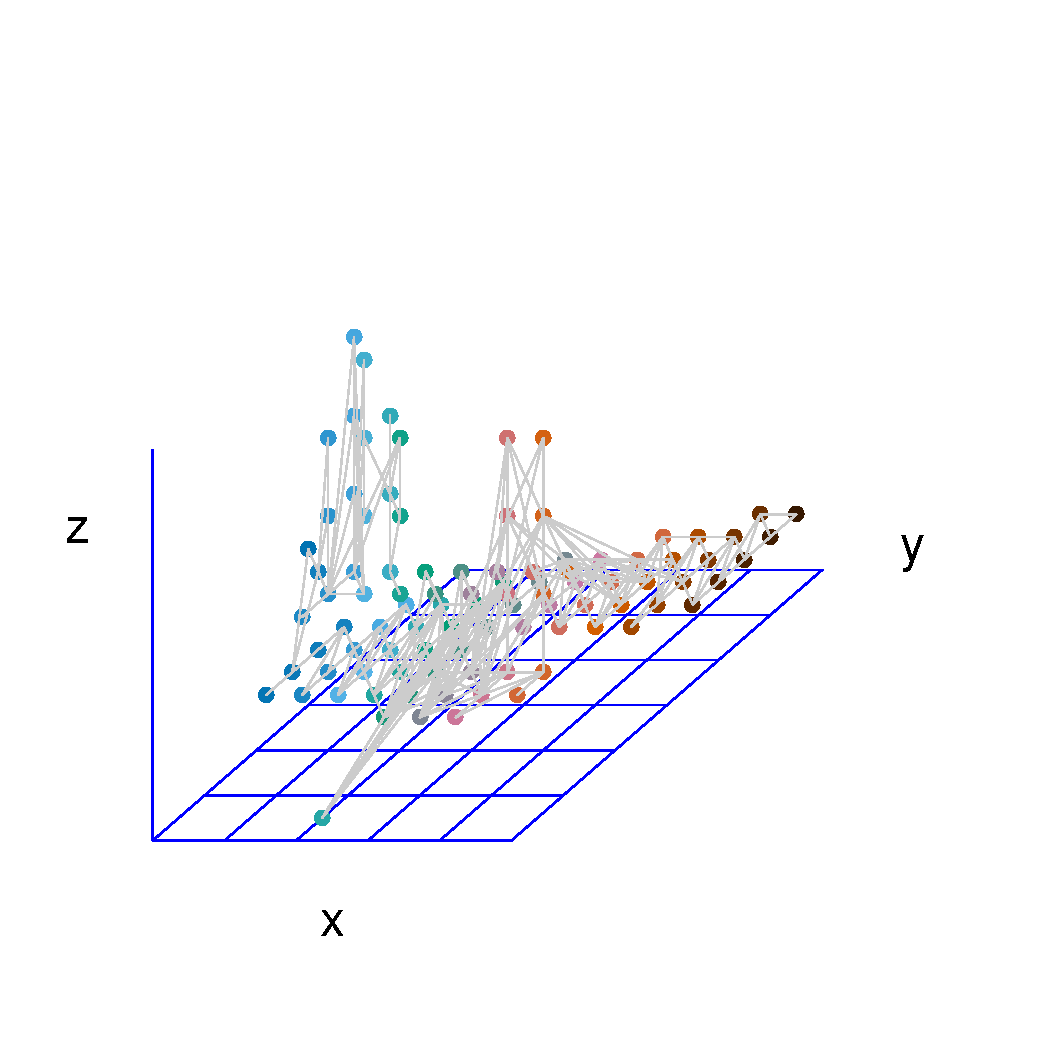
\includegraphics[width=2in]{../Figure/intro.pdf}	
	\label{fig:intro}
\end{figure}
We introduce a concept of each node's location over their underlying network to bring up the problem of testing independence between distance in terms of network in distance-based test. 
\subsection*{2. Multiscale Generalized Correlation}

\begin{figure}[H]
	\centering
	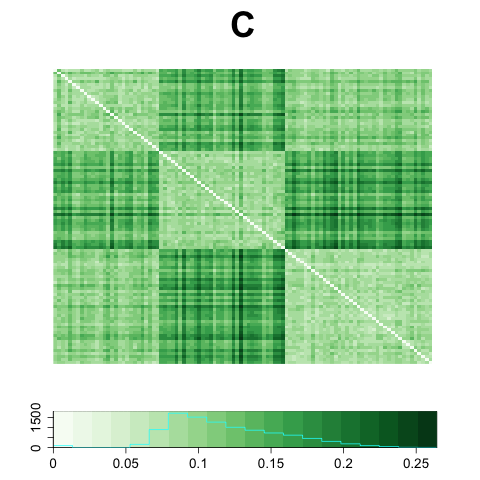
\includegraphics[width=1.5in]{../Figure/C.png}
	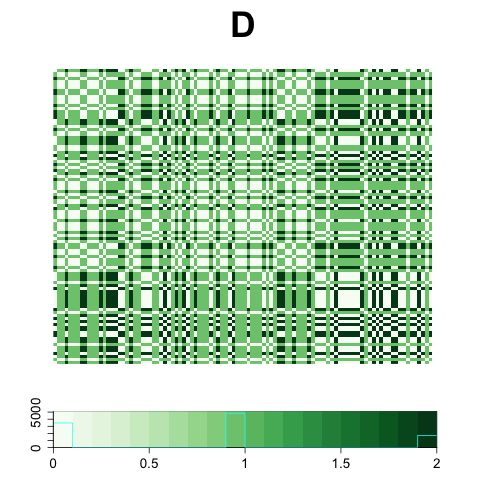
\includegraphics[width=1.5in]{../Figure/D.png}
	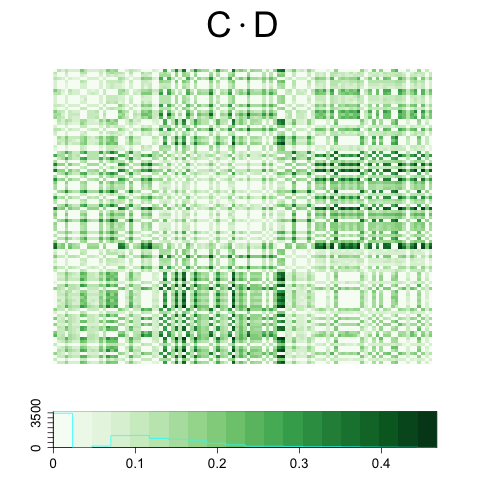
\includegraphics[width=1.5in]{../Figure/CD.png}
	
	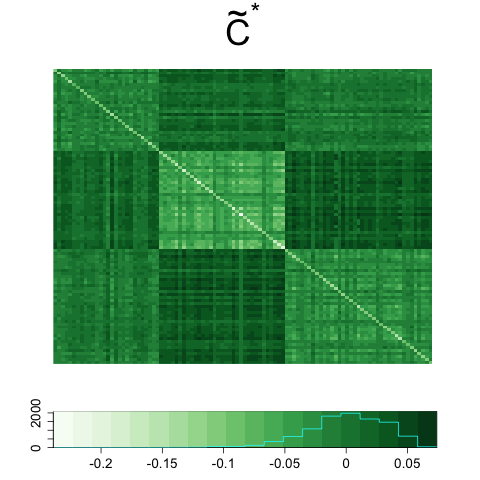
\includegraphics[width=1.5in]{../Figure/tildeCtrunc.png}
	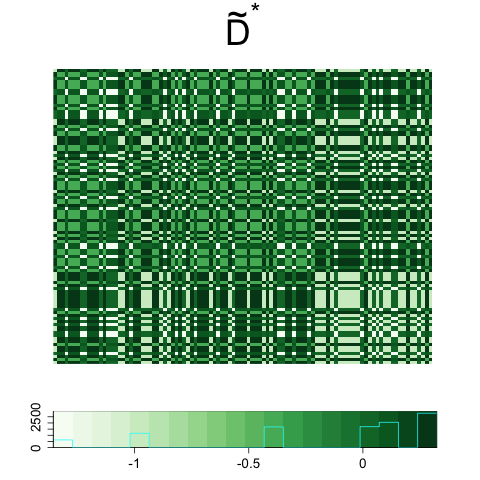
\includegraphics[width=1.5in]{../Figure/tildeDtrunc.png}
	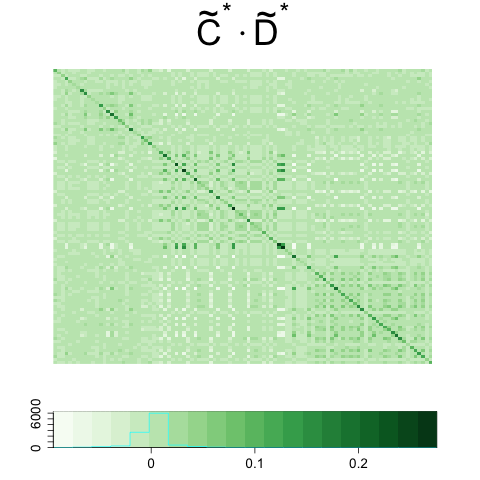
\includegraphics[width=1.5in]{../Figure/tildeCDtrunc.png}
	\label{fig:MGCmatrices}
\end{figure}	

As an efficient distance-based test in existence of nonlinear dependency and high-dimensionality, we adopt using local scale distance correlation which truncates each component of distance matrices up to a certain rank.

\subsection*{3. Problems in adopting  valid distance metric defined over network}

\begin{figure}[H]
	\centering
	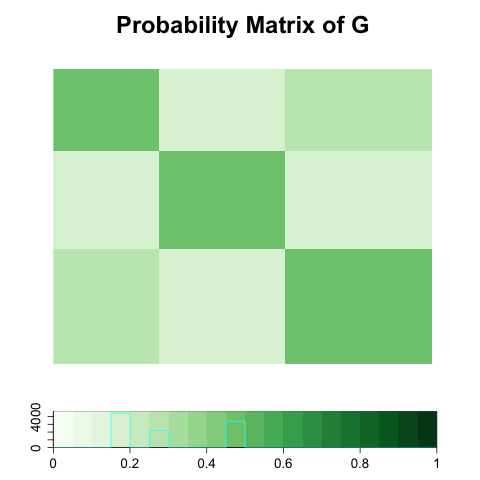
\includegraphics[width=1.5in]{../Figure/pmat.png}
	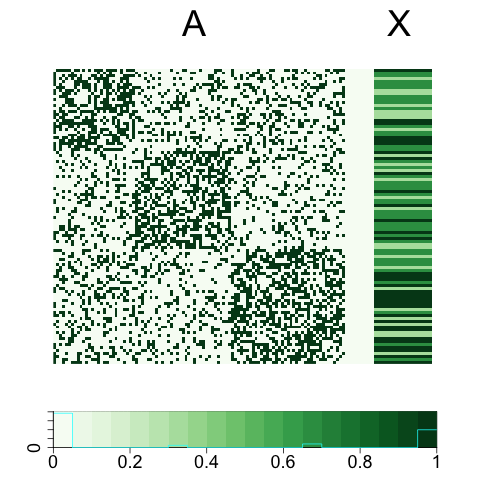
\includegraphics[width=1.5in]{../Figure/Amat.png}
	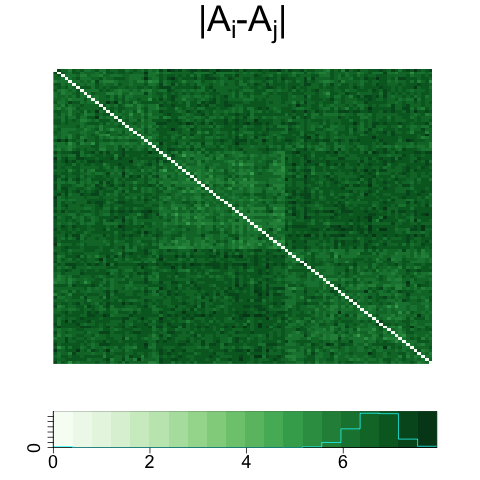
\includegraphics[width=1.5in]{../Figure/distA.png}
	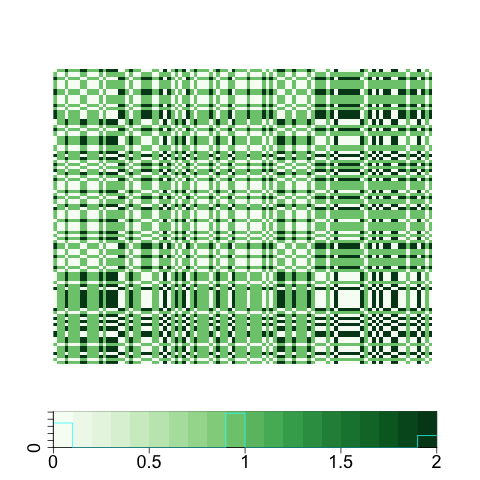
\includegraphics[width=1.5in]{../Figure/distX.png}
	\label{fig:matrics}
\end{figure}	
  
Every information on edge distribution is denoted in an adjacency matrix so we can consider its Euclidean distance matrix as an ingredient of the test statistics as well as that of nodal attributes.
  
\subsection*{4. demonstrate the validity of diffusion matrix } 

\begin{figure}[H]
	\centering
	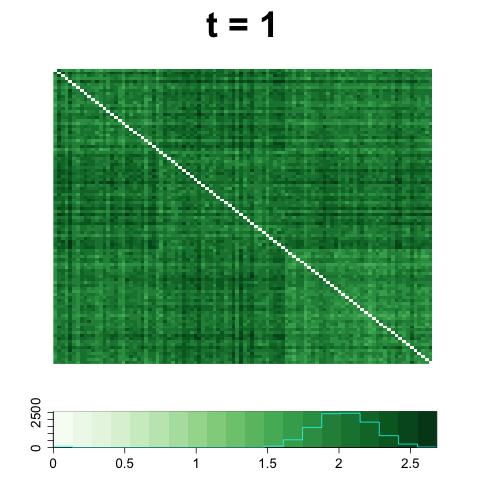
\includegraphics[width=1.5in]{../Figure/Dx1.png}
	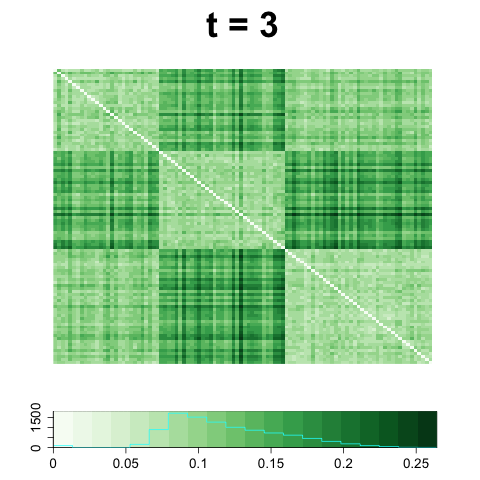
\includegraphics[width=1.5in]{../Figure/Dx3.png}
	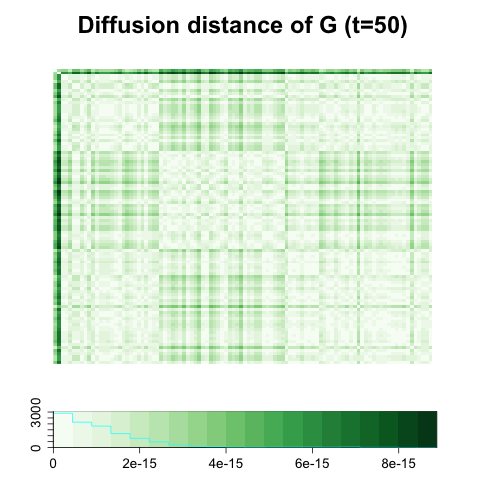
\includegraphics[width=1.5in]{../Figure/Dx50.png}
	\label{fig:diffusions}
\end{figure}	

Out of concerns on theoretical and also practical shortcomings of using an adjacency matrix, we introduce a one-parameter family of network metrics called \textit{diffusion matrix} which keeps every information of adjacent relation and also effectively captures the clustering of networks. 

\subsection*{5. Introducing the simulation study}

\begin{figure}[H]
	\centering
	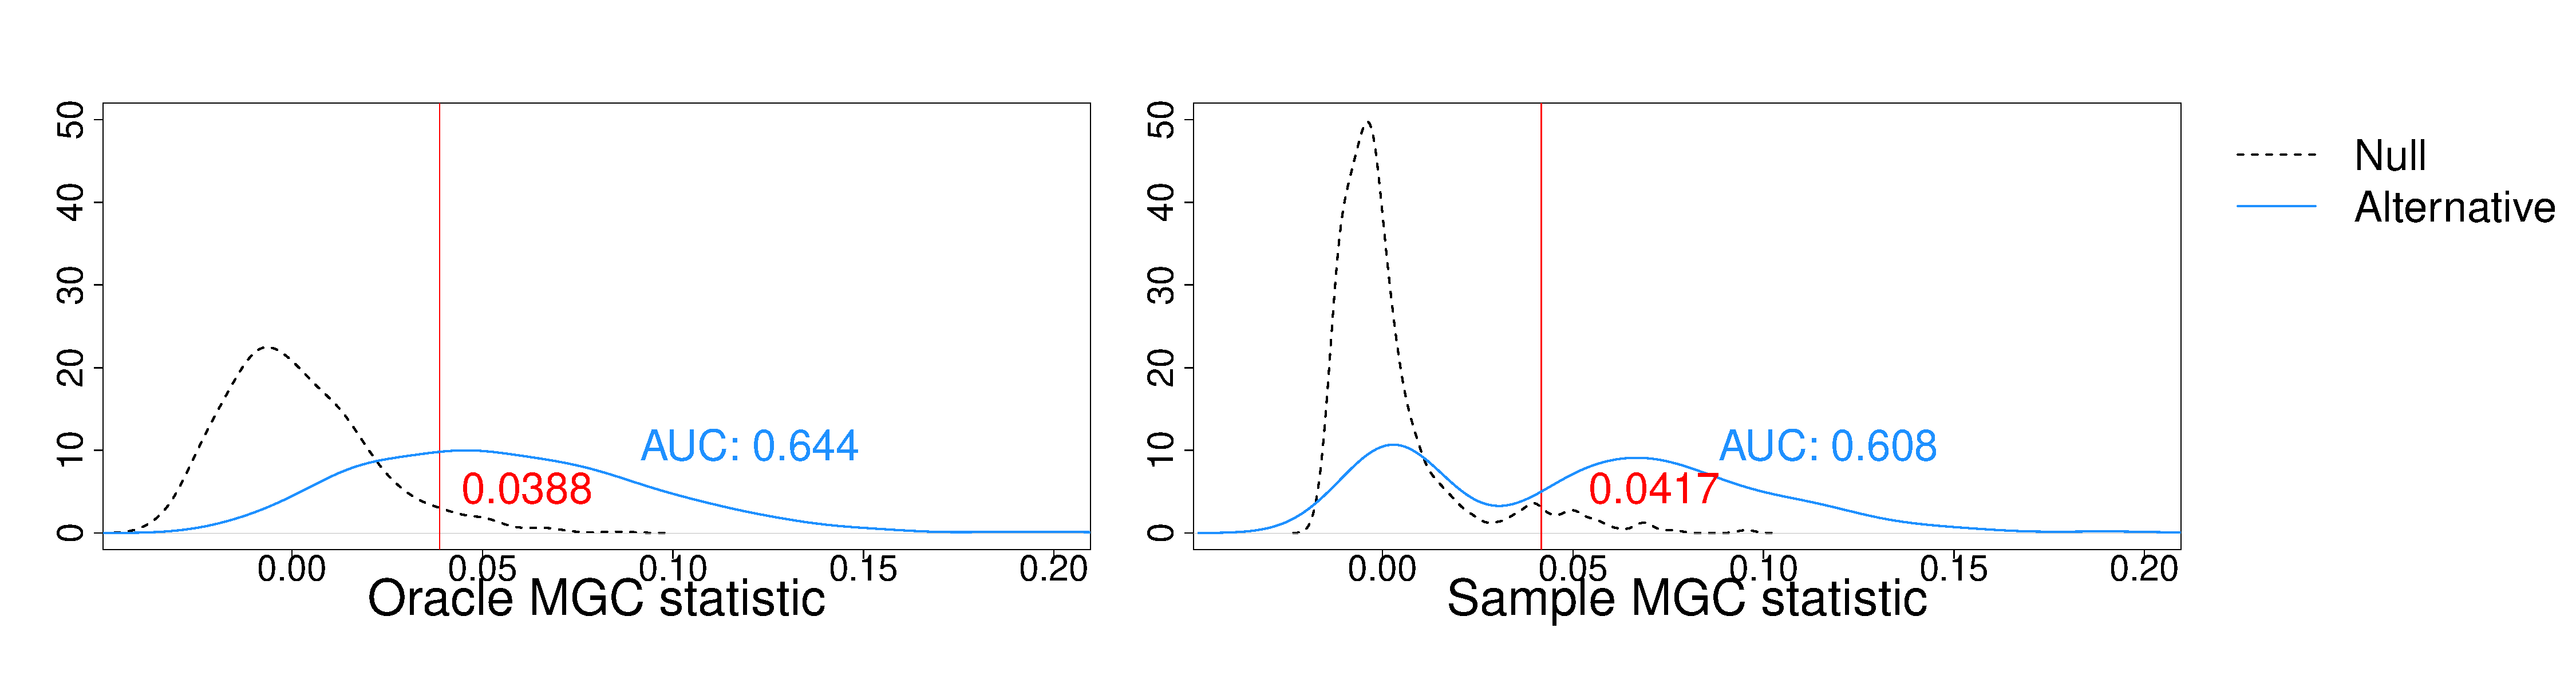
\includegraphics[width=6in]{../Figure/density.pdf}
	\label{fig:density}
\end{figure}	
 
 Throughout the simulation study, we are going to make a comparison between the proposed statistics from null simulated networks and also attribute-dependent simulated networks to calculate the empirical power, based on \texttt{Oracle MGC} and \texttt{Sample MGC}.
 
 
\subsection*{6. Simplest Stochastic Block Model}
 
\begin{figure}[H]
	\centering
	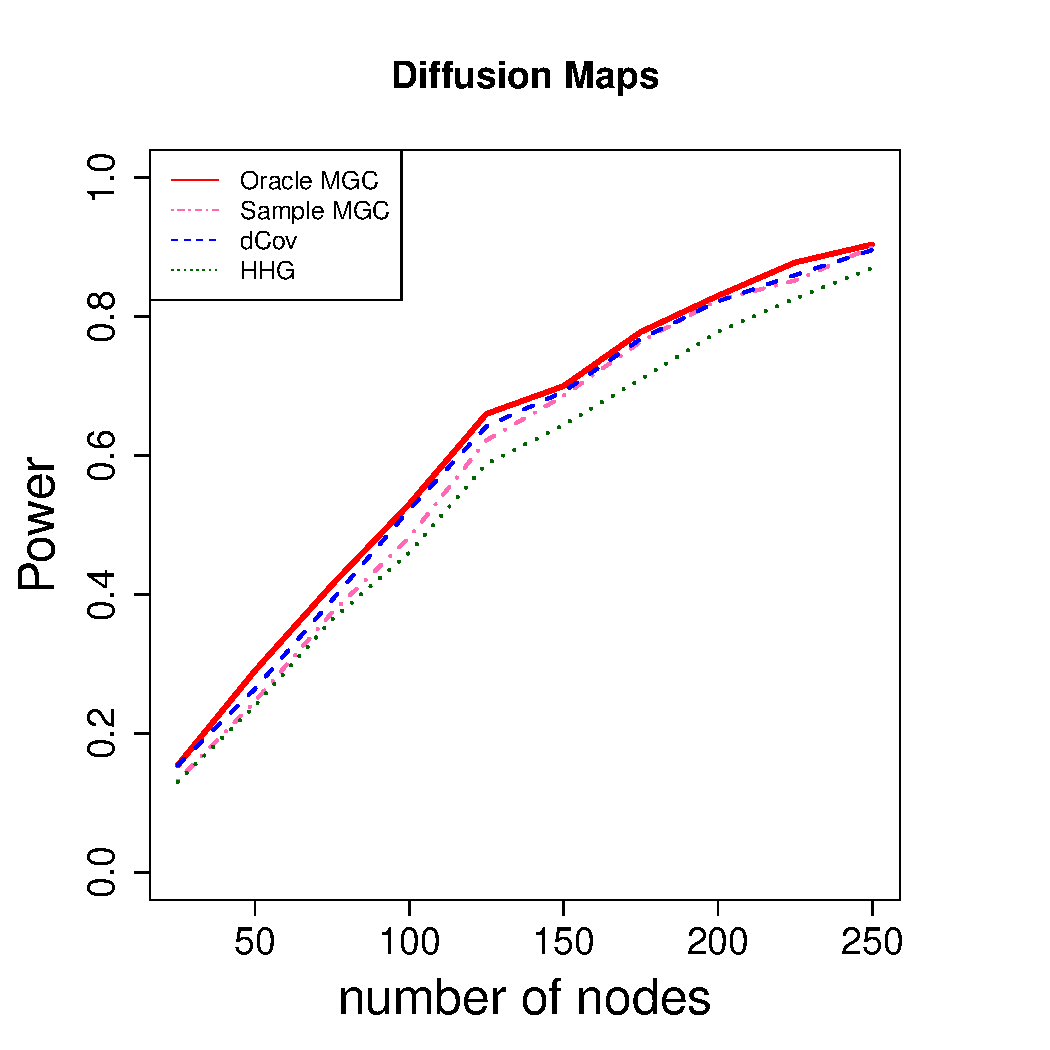
\includegraphics[width=6in]{../Figure/twoSBM.pdf}
	\label{fig:twoSBM}
\end{figure}

First simplest SBM with two blocks illustrates the typical case of linear-dependence so that we have similar results for each distance-based tests as well as \texttt{FH}-test.


\subsection*{7. Stochastic Block Model with non-linearly Dependent Attributes}

\begin{figure}[H]
	\centering
	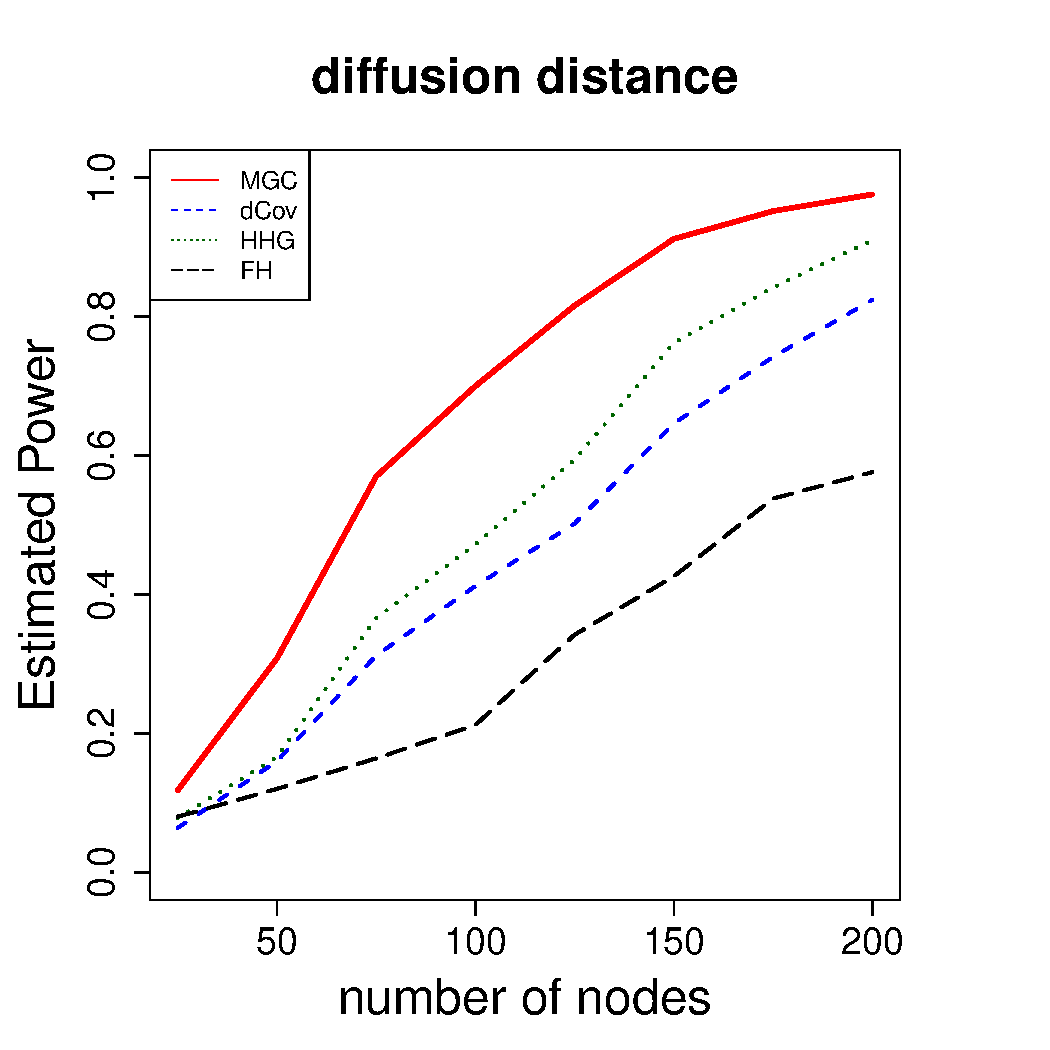
\includegraphics[width=6in]{../Figure/ThreeSBM.pdf}
	\label{fig:Three}
\end{figure}	

Next SBM is our punch line that \texttt{MGC} shows its superiority over other statistics especially in diffusion maps metrics and also results higher power in estimated latent position metric than \texttt{FH}.

\subsection*{8. Superiority of the proposed method under non-linear dependency}

\begin{figure}[H]
	\centering
	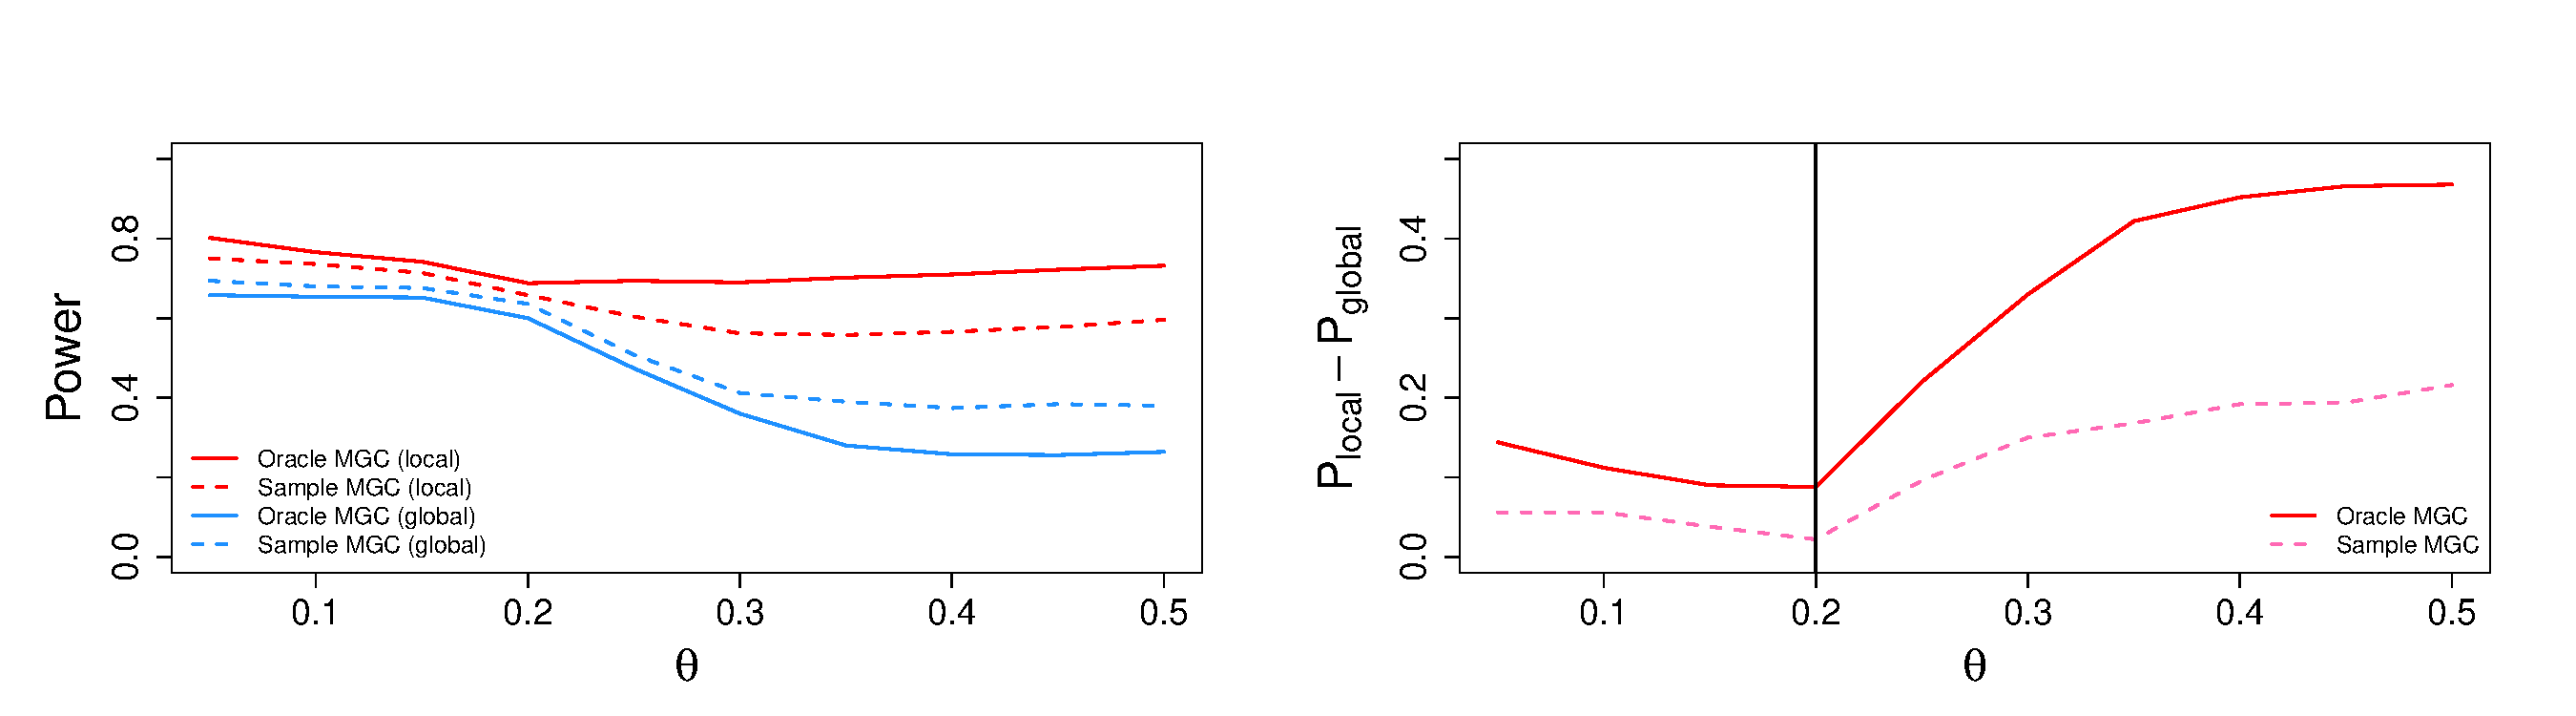
\includegraphics[width=5in]{../Figure/powerplot.pdf}
	\label{fig:powerplot}
\end{figure}

This plot deeps into when exactly our proposed tests exerts better performance; in the existence of non-linearity which can be formalized into conditional distribution of $A_{ij}$ given Euclidean distance between $\mathbf{X}_{i}$ and $\mathbf{X}_{j}$.

\subsection*{9. Degree-corrected SBM with increased variability in node distribution}	

\begin{figure}[H]
	\centering
	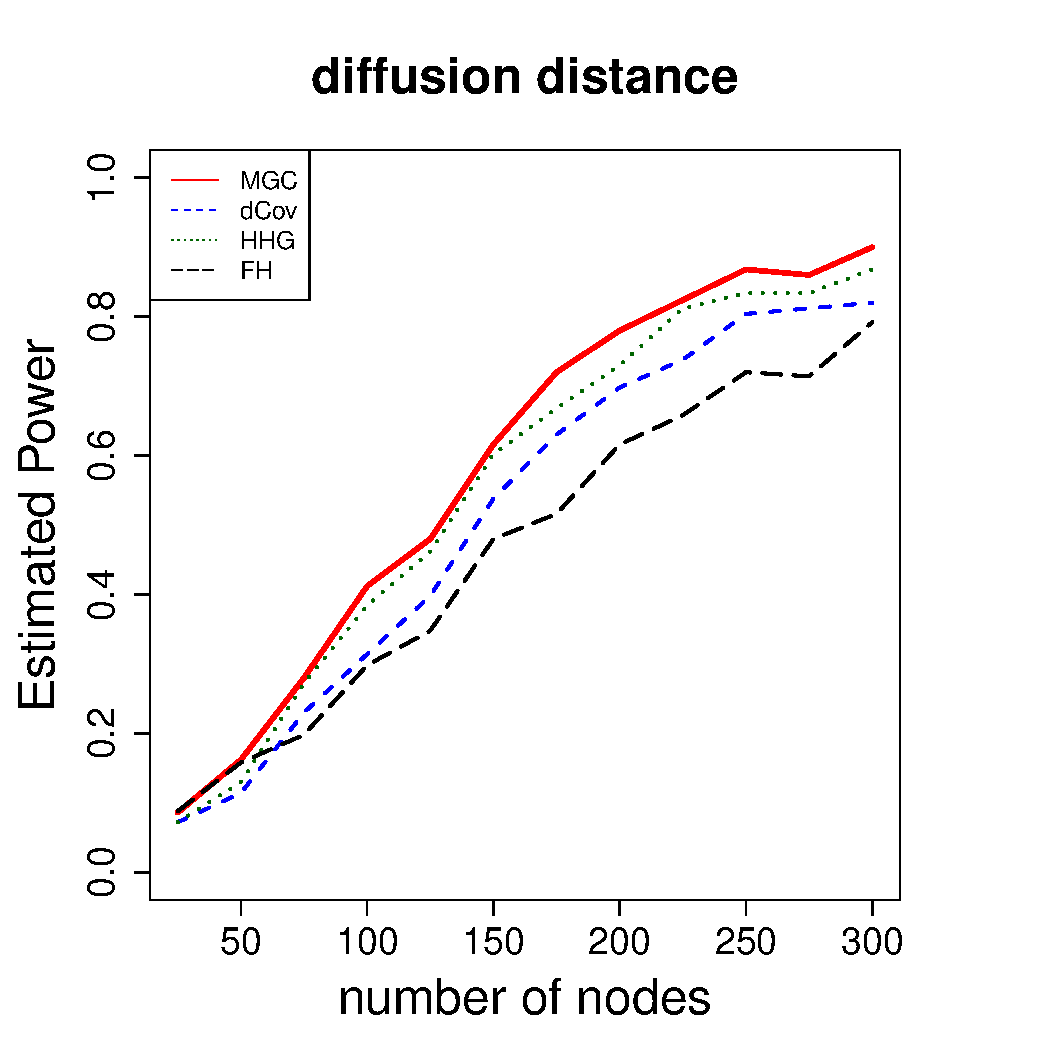
\includegraphics[width=6in]{../Figure/dcSBM.pdf}
	\label{fig:dcSBM}
\end{figure}	

Since previous two SBMs might not demonstrate the real example, we introduce a SBM but with increase variability in edge distribution and especially claim the improved power of diffusion maps when variance in an adjacency matrix is relatively higher.



\subsection*{10. Validity of the method even under competitor's model}

\begin{figure}[H]
	\centering
	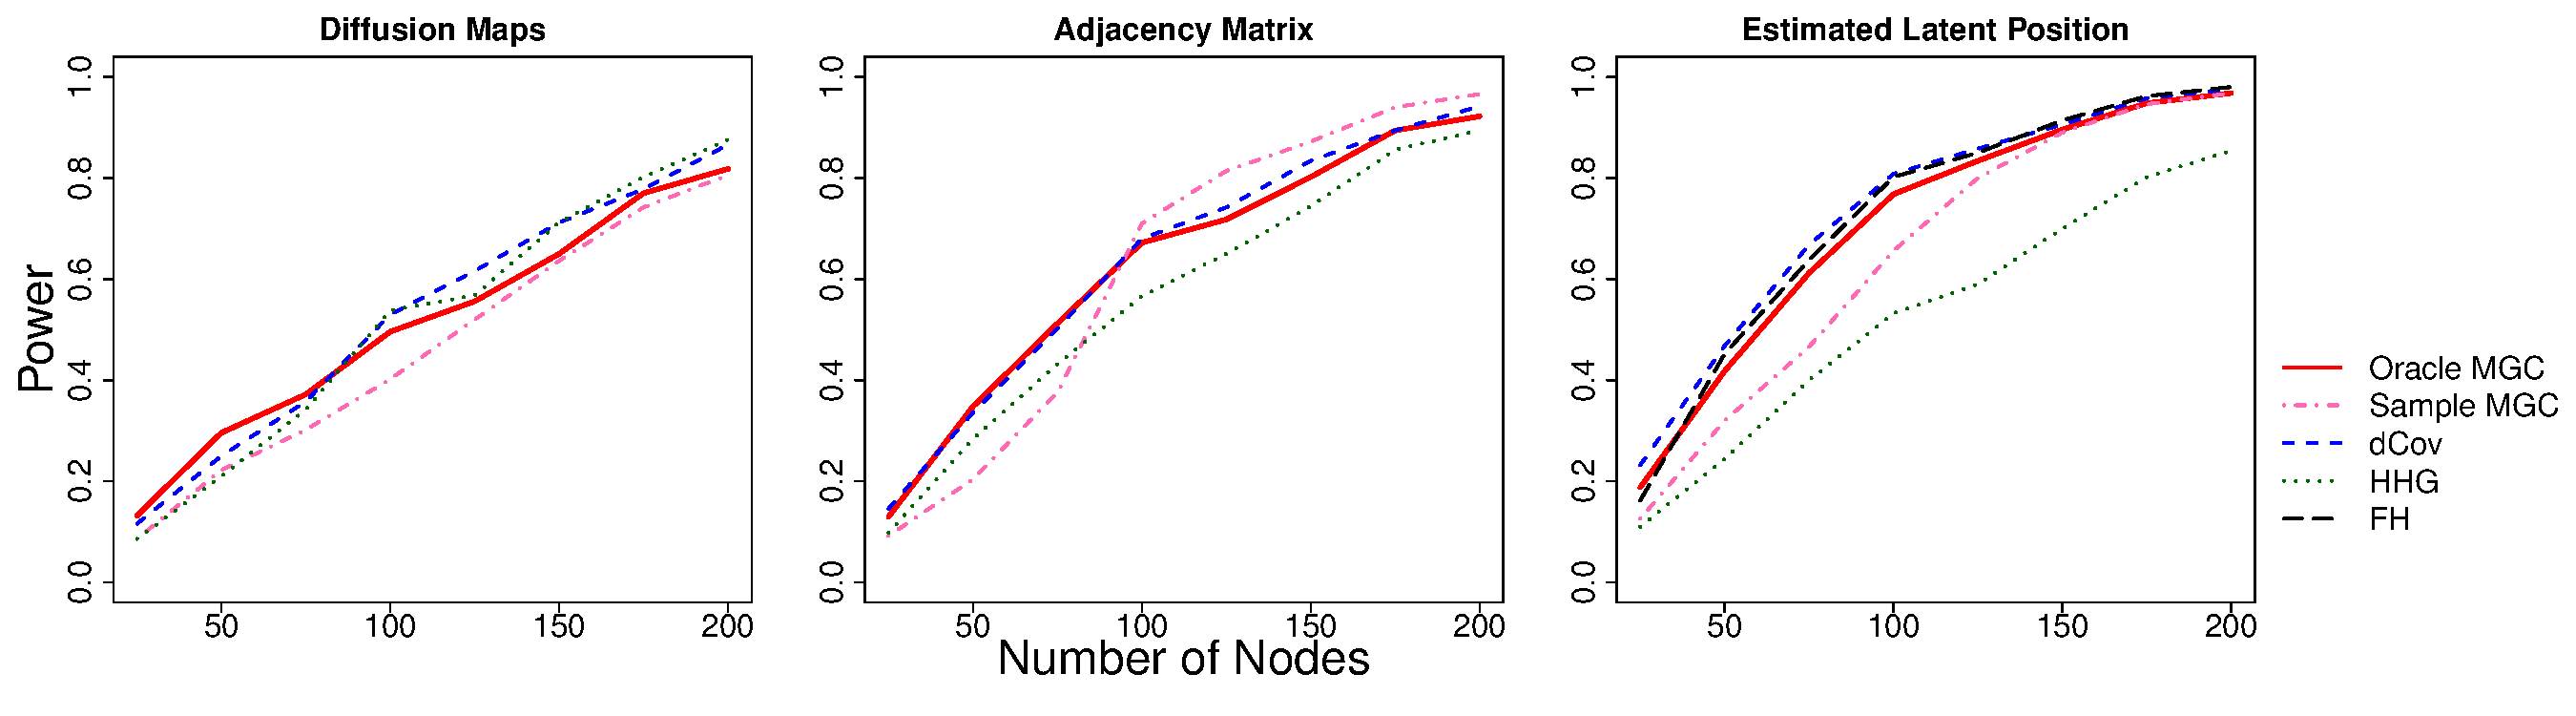
\includegraphics[width=6in]{../Figure/ame.pdf}
	\label{fig:ame}
\end{figure}	

However it would be fair to include others' mode-based tests and we can still suggest using estimated latent factors when the model is correct; but within that metrics our method does as good as their method. 

\subsection*{11. Node Contribution}


\begin{figure}[H]
	\centering
	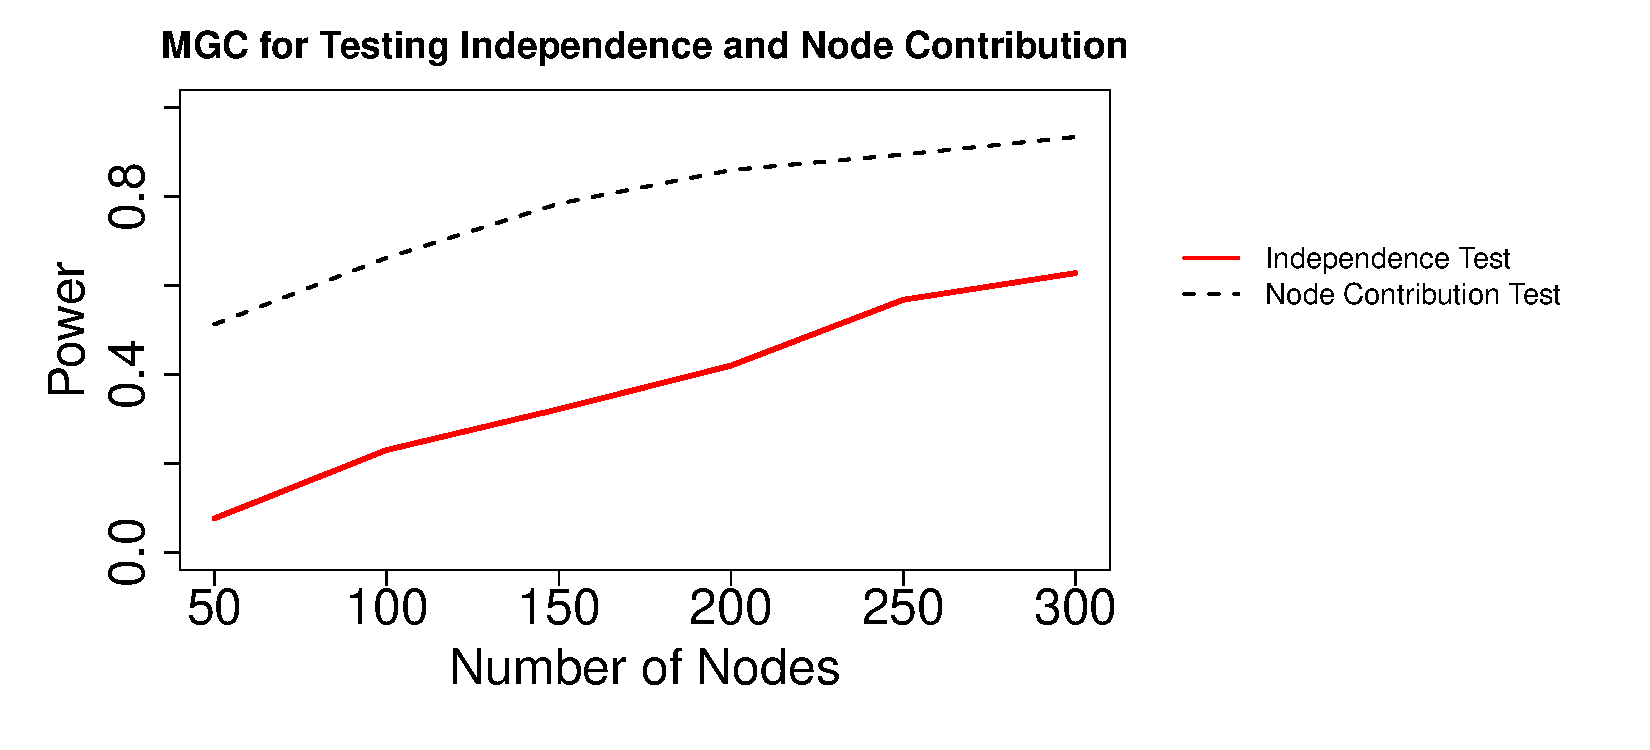
\includegraphics[width=6in]{../Figure/nodecontri.pdf}
	\caption{Change of empirical power and inclusion rate at each total sample size $n$. You can see that inclusion rate of $c(v)$ increases as empirical power of \texttt{MGC} increases.}
	\label{fig:contribution}
\end{figure}


\end{document}